\documentclass{article}

%===============================
%
%          📦 Paquetes
%
%===============================

% === Configuración del documento y tipografía ===
\usepackage[a4paper, top=3cm, bottom=2.5cm, left=2.5cm, right=2.5cm]{geometry}
\usepackage[spanish]{babel}
\usepackage[utf8]{inputenc}

% === Gráficos y representaciones visuales ===
\usepackage{tikz}
\usepackage{pgfplots}
\pgfplotsset{compat=1.18}
\usepackage{graphicx}
\usepackage{subcaption}

% === Estilo y personalización ===
\usepackage{titling}
\usepackage{titlesec}
\usepackage{tocloft} 
\usepackage{fancyhdr}
\usepackage{setspace}
\usepackage{caption}

% === Matemáticas y símbolos ===
\usepackage{amsmath}
\usepackage{amssymb}
\usepackage{cancel}

% === Estructura y disposición del contenido ===
\usepackage{array}
\usepackage{multicol}
\usepackage{float}
\usepackage{indentfirst}
\usepackage{enumitem}

% === Hipervínculos y referencias ===
\usepackage[nottoc]{tocbibind}
\usepackage{hyperref}

%===============================
%
%          ⬆️⬇️ Cabeceras
%
%===============================

\pagestyle{fancy}
\fancyhf{}
\fancyhead[L]{
\includegraphics[width=2cm]{assets/logo.png}}
\fancyhead[R]{\textit{Universidad Tecnológica del Perú}}
\fancyfoot[R]{\thepage}
\setlength{\headheight}{22.9188pt}
\addtolength{\topmargin}{-5.64944pt}

%======================================
%
%          📑 Espaciado de Párrafos
%
%======================================

\setlength{\parskip}{1.5em}
\setlength{\parindent}{0pt}

%======================================
%
%          📕 Estrucura del título
%
%======================================

\title{
  \pagenumbering{gobble}
  
\includegraphics[width=5cm]{./assets/logo-utp.png} \\
  \vspace{1cm}
  \textbf{Universidad Tecnológica del Perú} \\
  \vspace{2cm}
  \textbf{INFORME TÉCNICO} \\
  \textbf{APLICATIVO DE MONITOREO DE LOS EFECTOS DE LA VARIACIÓN EN LA TEMPERATURA SUPERFICIAL DEL MAR EN EL NDVI Y SU CORRELACIÓN.} \\
  \vspace{1cm}
}
\author{
  \begin{tabular}{ll}
    \textbf{Huatay Salcedo, Luis} & \texttt{u24218809@utp.edu.pe} \\
  \end{tabular} \\\\
}

\begin{document}
\maketitle

%======================================
%
%          📚 Inicio del documento
%
%======================================

\newpage

% Inicio de la numeración de páginas (desde aquí)
\pagenumbering{arabic}
\setcounter{page}{2}  

\tableofcontents
\thispagestyle{fancy}

% Introducción
\vspace*{\fill}

\section{Introducción}

  El presente proyecto tiene como finalidad aplicar la Metodología de Gestión de Proyectos Clásica, siguiendo el marco de trabajo propuesto por el Project Management Institute (PMI) y utilizando herramientas del Framework del PMBOK. Durante la primera parte de la unidad, se desarrollará un marco predictivo para la gestión de un proyecto empresarial, abarcando las fases de Iniciación y Planificación.

  Para ello, se seleccionará una empresa y área específica, describiendo su misión, visión y objetivos estratégicos, así como el alineamiento del proyecto con dichos objetivos. Posteriormente, se documentarán los procesos de iniciación (objetivos, alcance inicial, gestión de interesados y acta de constitución) y planificación (gestión de integración, alcance, cronograma, costes, calidad, recursos, comunicaciones, riesgos y adquisiciones).

  Finalmente, se presentará un informe detallado que incluya todos los elementos mencionados, demostrando la capacidad de aplicar la metodología de gestión de proyectos en un entorno empresarial real.

\vspace*{\fill}

% Capítulo 1
\section{Especificaciones Técnicas }

  En esta sección se detallan las especificaciones técnicas del proyecto, incluyendo los materiales y componentes utilizados, así como la descripción de los algoritmos que se implementaron en el sistema para la obtención de los insumos geoespaciales necesarios para el cálculo de la correlación de los datos.

  \subsection{Descripción del proyecto}

    El proyecto consiste en la implementación de un aplicativo desarrollado y deplegado en la plataforma Google Earth Engine, que permita monitorear los efectos de la variación en la temperatura superficial del mar en el Índice de Vegetación de Diferencia Normalizada (NDVI) así como con información del índice costero el niño (ICEN) y su correlación. Para ello se utilizan imagenes satelitales Sentinel2 de la misión Copernicus de la agencia espacial europea (ESA), las cuales son procesadas y analizadas en la plataforma Google Earth Engine.

  \subsection{Términos y definiciones}

    \begin{itemize}
      \item \textbf{Índice de Vegetación de Diferencia Normalizada (NDVI):} Es un índice que se utiliza para determinar la cantidad de vegetación que hay en un área determinada. Se calcula a partir de la diferencia entre el valor del infrarrojo cercano y el rojo, dividido por la suma de estos dos valores.
      \item \textbf{Índice Costero el Niño (ICEN):} Es un índice que se utiliza para determinar la presencia de eventos de El Niño en la región costera del Perú. Se calcula a partir de la temperatura superficial del mar y la presencia de anomalías térmicas en la región.
      \item \textbf{Google Earth Engine:} Es una plataforma desarrollada por Google que permite el procesamiento y análisis de información geoespacial a gran escala y de uso libre.
      \item \textbf{Sentinel2:} Es una misión de la Agencia Espacial Europea (ESA) que proporciona imágenes satelitales de alta resolución y de uso libre. Esta misión está compuesta por dos satélites, Sentinel-2A y Sentinel-2B, que orbitan la Tierra cada 5 días.
      \item \textbf{NOAA - MODIS:} Es un sensor de imágenes satelitales que proporciona información sobre la temperatura superficial del mar y otros parámetros oceánicos. Este sensor es operado por la Administración Nacional Oceánica y Atmosférica (NOAA) de los Estados Unidos.
      \item \textbf{Asset:} Es un recurso geoespacial que se almacena en la plataforma Google Earth Engine. Los assets pueden ser imágenes, capas vectoriales, tablas, entre otros.
      \item \textbf{Script:} Es un conjunto de instrucciones que se ejecutan en la plataforma Google Earth Engine para realizar un procesamiento específico. Los scripts pueden ser escritos en JavaScript o Python.
      \item \textbf{GitHub Actions:} Es una herramienta de integración continua y entrega continua (CI/CD) que permite automatizar tareas en GitHub. Esta herramienta permite ejecutar scripts de Python en un intervalo de tiempo determinado, lo que permite mantener la información actualizada.
      \item \textbf{TSM:} Es un acrónimo de temperatura superficial del mar. Este parámetro se utiliza para determinar la presencia de anomalías térmicas en la región costera del Perú.
      \item \textbf{Correlación:} Es una medida estadística que indica la relación entre dos variables. En este caso, se utiliza para determinar la relación entre el NDVI y la TSM. La correlación se calcula utilizando el algoritmo de Pearson, que permite obtener un coeficiente de correlación entre -1 y 1. 
    \end{itemize}
  \subsection{Materiales y componentes}

    \begin{itemize}
      \item \textbf{Google Earth Engine:} Plataforma de procesamiento y análisis de imágenes satelitales.
      \item \textbf{Sentinel2:} Imágenes satelitales de la misión Copernicus de la agencia espacial europea (ESA).
      \item \textbf{Javascript:} Lenguaje de programación utilizado para el desarrollo del aplicativo. 
    \end{itemize}

  \subsection{Algoritmos implementados}
  
    %%\begin{enumerate}[label=\thesubsection.\arabic*, leftmargin=1.5cm]
      \subsubsection{\textbf{Selector de área de interés}}
      
      La primera parte del aplicativo consiste en seleccionar el área de interés en la que se desea realizar el análisis. Para ello se le brinda al usuario un pánel principal donde escoger en tres fases la región de interés. Mediante la selección se un departamento y provincia este dispone de una lista de distritos que son pretenecientes a dicha provincia. Finalmente se selecciona un distrito y se muestra en el mapa la región seleccionada.

      La información vectorial de los departamentos, provincias y distritos se obtiene de la plataforma de geodatos del Instituto Nacional de Estadística e Informática (INEI) del Perú. Este se encuentra actualizado al año 2023 y se encuentra disponible en la plataforma oficial mediante el siguiente link \href{https://ide.inei.gob.pe/#capas/}{https://ide.inei.gob.pe/\#capas/}.

      \subsubsection{\textbf{Cálculo del área de cobertura agrícola permanente.}}
      
      Para calcular el área de cobertura agrícola permanente se utilizan imágenes provenientes del satelite Sentinel2 de la misión Copernicus de la agencia espacial europea (ESA). Estas imágenes son procesadas y analizadas en la plataforma Google Earth Engine. Para evitar problemas de nubes y sombras se aplica un filtro del 10\% de nubes, lo que permite obtener imágenes óptimas. Posteriormente tomando como referencia el área escogida mediante el la primera fase, se restringe el procesamiento a dicha área lo que permite mejorar los tiempos de cómputo.

      De entre las imagenes se toma una muestra por mes, lo que equivale a 12 imagenes obtenidas por año, éste último parámetro puede cambiar para mejorar la presición de la segmentación agrícola, en este punto se procesan solo los píxeles que mantienen un valor de NDVI mayor o igual a $0.55$, finalmente este resultado pasa por un proceso de conversión a vectores poligonales, lo que permite obtener así, regiones que se considere cobertura agrícola permanente.

      \subsubsection{\textbf{Integración con la información del ICEN.}}
      
      La información del índice costero el niño (ICEN) se obtiene a partir del repositorio de datos de la Subdirección de Ciencias de la Atmósferea e Hidrósfera del Instituto Geofísico del Perú, disponible en la plataforma oficial mediante el siguiente link: \href{http://met.igp.gob.pe/datos/ICEN.txt}{http://met.igp.gob.pe/datos/ICEN.txt}.
      
      Esta información se encuentra disponible en formato de texto plano y contiene datos de anomalías térmicas en la temperatura superficial del mar (TSM).

      Para hacer uso de los datos dentro del algoritmo de procesamiento en la aplicación, se desarrolló un proceso basado en la solicitud de datos mediante un script en Python, que realiza la descarga y almacenamiento en un archivo CSV, el cuál se guarda en un repositorio de GitHub. Este archivo CSV es posteriormente inyectado a la plataforma de Google Earth Engine como un asset nuevo. Todo este proceos es automatizado gracias al servicio de GitHub Actions, el cuál permite ejecutar scripts de Python en un intervalo de tiempo determinado. En este caso se ejecuta cada 24 horas, lo que permite mantener la información actualizada.

      \subsubsection{\textbf{Cálculo de anomalía térmica en la TSM - MODIS.}}
      
      A fin de poder utilizar información actualizada, se utiliza el sensor MODIS de la Administración Nacional Oceánica y Atmosférica (NOAA) de los Estados Unidos. Este sensor proporciona información sobre la temperatura superficial del mar y otros parámetros oceánicos. Este asset se utiliza mediante los servicios de Google Earth Engine, el cuál permite acceder a información de diferentes sensores y misiones espaciales. En este caso se utiliza el sensor MODIS Aqua, que proporciona información diaria sobre la temperatura superficial del mar.

      Para el cálculo de la anomalía térmica en la TSM, se utiliza un algoritmo que calcula la diferencia entre la temperatura superficial del mar y la media de los últimos 30 años. Con esto se obtiene una lista del registro histórico de la temperatura superficial del mar de los últimos 15 años, información que servirá para entender mejor el comportamiento histórico del NDVI frente a dichas anomalías.

      \subsubsection{\textbf{Registro histórico del NDVI vs TSM.}}
      
      Al seleccionar un mes en específico, se calcula el registro histórico de los niveles NDVI en las zonas devueltas por el cálculo de la cobertura agrícola permanente que se toman a modo de área de muestra, se realiza el cálculo de la media mensual del año en curso y de 14 años anteriores, posteriormente se comparan con el resgistro de la TSM de dos meses antes, tiempo que se considera promedio sobre el cual se perciben los efectos de la anomalía en la TSM. Finalmente cada registro es devuelto en una lista que se toma como entrada de datos para el procesado de un gráfico comparativo.

      Esta información ayuda a poder entender el comportamiento del NDVI en dichas zonas a lo largo de los años, lo que permite identificar patrones y tendencias en el comportamiento del NDVI frente a las anomalías térmicas en la TSM. Esta información es útil para la toma de decisiones en la gestión de riesgos y la planificación agrícola.
      
      \subsubsection{\textbf{Cálculo de la correlación entre el NDVI y la TSM.}}
      
      La correlación entre el NDVI y la TSM se calcula de manera particular para cada caso del distrito escogido y es realizado tomando los registros de eventos extremos, evento de mediana y baja intensidad, así como eventos normales. Utilizando el algoritmo de Pearson, se obtiene el coeficiente de correlación entre el NDVI y la TSM. Este coeficiente varía entre -1 y 1, donde -1 indica una correlación negativa perfecta, 0 indica una ausencia de correlación y 1 indica una correlación positiva perfecta. 

      Este análisis permite determinar la vulnerabilidad de cada distrito seleccionado frente a eventos extremos así como el mapeo de estos, información que puede ser utilizada para la toma de decisiones en la gestión de riesgos y la planificación agrícola.
      
      

    %%\end{enumerate}

% Capítulo 2
\section{Manual de usuario aplicativo GEE}

En el contexto presente, el manual de usuario del aplicativo GEE se presenta como una guía integral para la utilización efectiva de la herramienta. Este manual está diseñado para facilitar la comprensión y el uso del aplicativo, proporcionando instrucciones claras y concisas sobre su funcionamiento.

El aplicativo GEE, desarrollado en Google Earth Engine, permite la visualización y análisis de datos geoespaciales relacionados con la temperatura superficial del mar (TSM) y su correlación con el índice de vegetación de diferencia normalizada (NDVI). A través de este manual, los usuarios podrán familiarizarse con las funcionalidades del aplicativo, así como con los pasos necesarios para llevar a cabo un análisis efectivo de los datos disponibles.

\subsection{Descripción de la interfaz}

La interfaz del aplicativo GEE está diseñada para ser intuitiva y fácil de usar. En $[1]$, se presenta el mapa espacio donde los usuarios pueden visualizar el área de muestra de cobertura agrícola permanente, luego en $[2]$ se muestra el panel de opciones se detalla primero la entidad que presenta la herramienta seguido de información acerca del aplicativo. A continuación de ello se muestran los botones selectores de zona de estudio.

\begin{figure}[ht]
  \centering
  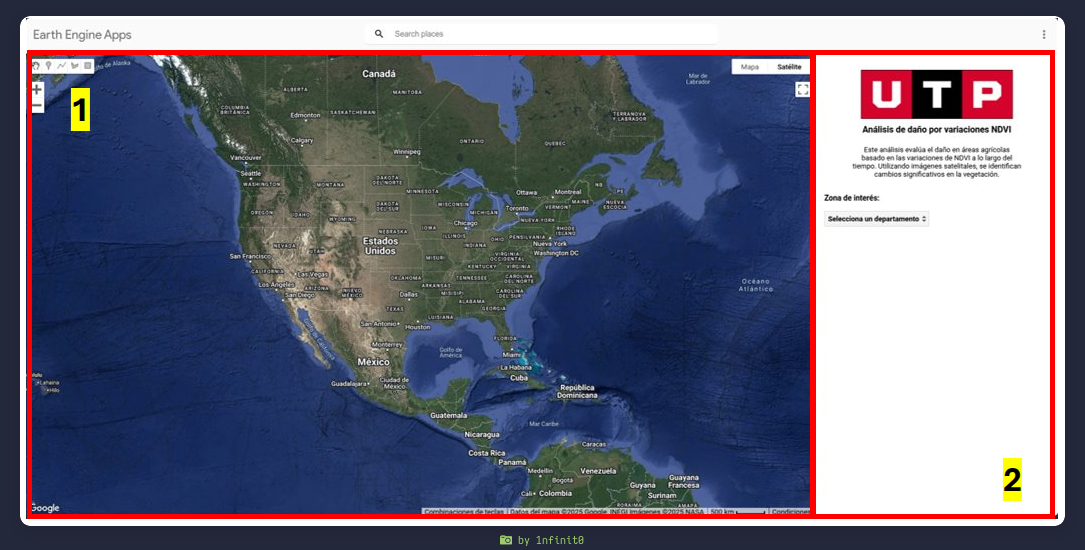
\includegraphics[width=\textwidth, trim=20px 25px 20px 20px, clip]{assets/canvas.png}
  \caption{Primera pantalla del aplicativo GEE.}
  \label{fig:canvas}
\end{figure}

\subsection{Uso del aplicativo}

El aplicativo GEE permite a los usuarios seleccionar un distrito dada una lista de departamentos y provincias. $[1]$.

Una vez seleccionada la zona de estudio, el aplicativo solicitará escoger un mes en específico, esta información servirá para poder realizar las operaciones descritas por los algoritmos mencionados. $[2]$.

\begin{figure}[ht]
  \centering
  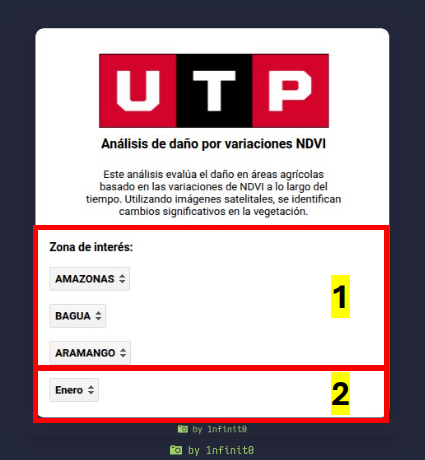
\includegraphics[width=7cm, trim=37px 38px 38px 50px, clip]{assets/panel.png}
  \caption{Panel de selección de área de interés}
  \label{fig:panel}
\end{figure}

\subsection{Interpretación de gráficos}

Una vez seleccionada la zona de estudio y el mes, el aplicativo generará 4 gráficos:

En $[1]$ se muestra el monitoreo del ICEN mensual en los últimos 12 registros que se hayan actualizado en la plataforma del IGP, esto con la finalidad de poder realizar un análisis de la tendencia del índice de calor en el área seleccionada. En $[2]$ se muestra el monitoreo la anomalía de TSM mensual en los últimos 12 meses desde el momento de consulta, esta información proporcionada por el sensor MODIS-AQUA.

\begin{figure}[ht]
  \centering
  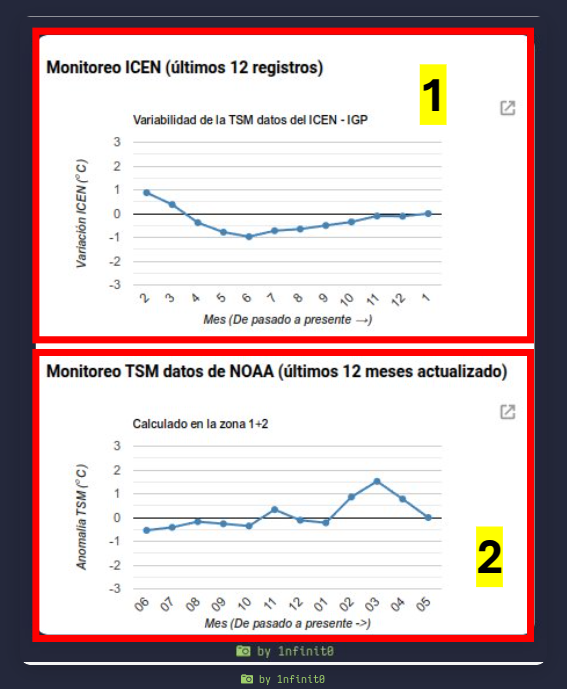
\includegraphics[width=7cm, trim=37px 48px 38px 32px, clip]{assets/grafico1.png}
  \caption{Gráficos de monitoreo de anomalía TSM}
  \label{fig:tsm}
\end{figure}

\newpage

En $[3]$ se muestra el monitoreo del NDVI del mes seleecionado y se compara con los niveles del mismo mes en los últimos 15 años, esto con la finalidad de poder realizar un análisis de la tendencia en comparación con los ciclos en los cuales ocurren estos fenómenos. Finalmente, en $[4]$ se muestra la correlación de estos valores en el área seleccionada, lo que pretende brindar una idea del nivel de vulnerabilidad de la zona de estudio ante el fenómeno climático.

\begin{figure}[ht]
  \centering
  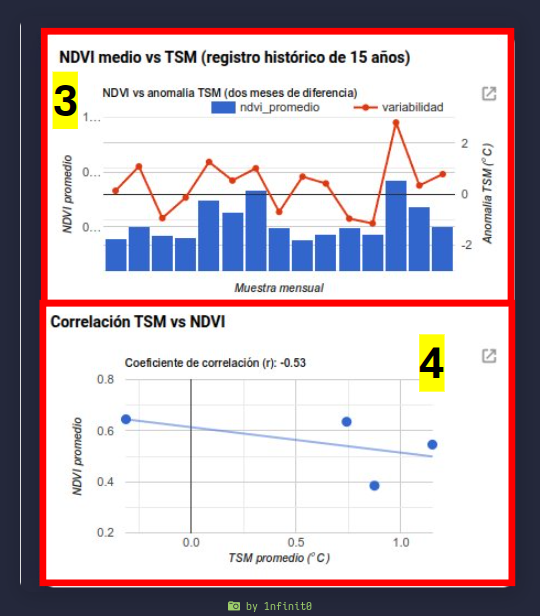
\includegraphics[width=8cm, trim=37px 29px 25px 25px, clip]{assets/correlacion.png}
  \caption{Gráficos de NDVI histórico y correlación}
  \label{fig:correlación}
\end{figure}

% Capítulo 3
\section{Comentarios}

  \subsection{Cobertura agrícola permanente}
  
    El cálulo para la obtención de la cobertura agrícola permanente pretende ser una correcta forma de poder tomar muestras de áreas que se consideren como tal para el desarrollo de los cálculos de de daño y su correlación con la TSM. Debido a la ténica de la teledetección es posible que no se tome el total del área que se considera cobertura agrícola permanente, pero si la suficiente para poder considerarse una muestra aceptable.

  \subsection{Registro histórico del NDVI}

    La comparación entre los valores NDVI de la cobertura agrícola permanente y la TSM, son información del mes seleccionado comparado con la TSM de dos meses anteriores al mes escogido. Si bien, esto permite poder entender el comportamiento del NDVI frente a la anomalía de temperatura, es importante entender que los cambios significativos refieren a los meses de mayor anomalía (diciembre - marzo) y no a los dos meses anteriores como se hace en el algoritmo. El enfoque de este algoritmo es poder entender el comportamiento del NDVI frente a la anomalía de temperatura 

\end{document}